
\documentclass[10pt]{beamer}
\usepackage{amsmath}
\usepackage{mathtools}
\usepackage{multimedia}
\usepackage{hyperref}


\usefonttheme{professionalfonts} % using non standard fonts for beamer
\usefonttheme{serif} % default family is serif
%\documentclass[12pt]{beamerthemeSam.sty}
\usepackage{epsf}
%\usepackage{pstricks}
%\usepackage[orientation=portrait,size=A4]{beamerposter}
\geometry{paperwidth=160mm,paperheight=120mm}
%DT favorite definitions
\def\LL{\left\langle}	% left angle bracket
\def\RR{\right\rangle}	% right angle bracket
\def\LP{\left(}		% left parenthesis
\def\RP{\right)}	% right parenthesis
\def\LB{\left\{}	% left curly bracket
\def\RB{\right\}}	% right curly bracket
\def\PAR#1#2{ {{\partial #1}\over{\partial #2}} }
\def\PARTWO#1#2{ {{\partial^2 #1}\over{\partial #2}^2} }
\def\PARTWOMIX#1#2#3{ {{\partial^2 #1}\over{\partial #2 \partial #3}} }

\def\rightpartial{{\overrightarrow\partial}}
\def\leftpartial{{\overleftarrow\partial}}
\def\diffpartial{\buildrel\leftrightarrow\over\partial}

\def\BS{\bigskip}
\def\BC{\begin{center}}
\def\EC{\end{center}}
\def\BN{\begin{enumerate}}
\def\EN{\end{enumerate}}
\def\BI{\begin{itemize}}
\def\EI{\end{itemize}}
\def\BE{\begin{displaymath}}
\def\EE{\end{displaymath}}
\def\BEA{\begin{eqnarray*}}
\def\EEA{\end{eqnarray*}}
\def\BNEA{\begin{eqnarray}}
\def\ENEA{\end{eqnarray}}
\def\EL{\nonumber\\}

\newcommand{\etal}{{\it et al.}}
\newcommand{\gbeta}{6/g^2}
\newcommand{\la}[1]{\label{#1}}
\newcommand{\ie}{{\em i.e.\ }}
\newcommand{\eg}{{\em e.\,g.\ }}
\newcommand{\cf}{cf.\ }
\newcommand{\etc}{etc.\ }
\newcommand{\atantwo}{{\rm atan2}}
\newcommand{\Tr}{{\rm Tr}}
\newcommand{\dt}{\Delta t}
\newcommand{\op}{{\cal O}}
\newcommand{\msbar}{{\overline{\rm MS}}}
\def\chpt{\raise0.4ex\hbox{$\chi$}PT}
\def\schpt{S\raise0.4ex\hbox{$\chi$}PT}
\def\MeV{{\rm Me\!V}}
\def\GeV{{\rm Ge\!V}}

%AB: my color definitions
%\definecolor{mygarnet}{rgb}{0.445,0.184,0.215}
%\definecolor{mygold}{rgb}{0.848,0.848,0.098}
%\definecolor{myg2g}{rgb}{0.647,0.316,0.157}
\definecolor{A}{rgb}{1.0,0.3,0.3}
\definecolor{B}{rgb}{0.0,1.0,0.0}
\definecolor{C}{rgb}{1.0,1.0,0.0}
\definecolor{D}{rgb}{0.5,0.5,1.0}
\definecolor{E}{rgb}{0.7,0.7,0.7}
\definecolor{abtitlecolor}{rgb}{1.0,1.0,1.0}
\definecolor{absecondarycolor}{rgb}{0.0,0.416,0.804}
\definecolor{abprimarycolor}{rgb}{1.0,0.686,0.0}
\definecolor{Red}           {rgb}{1,0.4,0.4}
\definecolor{Yellow}           {rgb}{1,1,0.0}
\definecolor{Grey}          {cmyk}{.7,.7,.7,0}
\definecolor{Blue}          {cmyk}{1,1,0,0}
\definecolor{Green}         {cmyk}{1,0,1,0}
\definecolor{Brown}         {cmyk}{0,0.81,1,0.60}
\definecolor{Silver}        {rgb}{0.95,0.9,1.0}
\definecolor{Sky}           {rgb}{0.07,0.0,0.2}
\definecolor{Darkbrown}     {rgb}{0.4,0.3,0.2}
\definecolor{40Gray}        {rgb}{0.4,0.4,0.5}
\usetheme{Madrid}


\setbeamercolor{normal text}{fg=Silver,bg=Sky}

%AB: redefinition of beamer colors
%\setbeamercolor{palette tertiary}{fg=white,bg=mygarnet}
%\setbeamercolor{palette secondary}{fg=white,bg=myg2g}
%\setbeamercolor{palette primary}{fg=black,bg=mygold}
\setbeamercolor{title}{fg=abtitlecolor}
\setbeamercolor{frametitle}{fg=abtitlecolor}
\setbeamercolor{palette tertiary}{fg=white,bg=Darkbrown}
\setbeamercolor{palette secondary}{fg=white,bg=absecondarycolor}
\setbeamercolor{palette primary}{fg=white,bg=40Gray}
\setbeamercolor{structure}{fg=abtitlecolor}

\setbeamerfont{section in toc}{series=\bfseries}

%AB: remove navigation icons
\beamertemplatenavigationsymbolsempty
\title[The phases of the Moon]{
  \textbf {The phases of the Moon}
}

\author [Astronomy 101]{Astronomy 101\\Syracuse University, Fall 2018\\Walter Freeman}

\date{\today}

\begin{document}



\frame{\titlepage}

\frame{\frametitle{\textbf{Announcements}}
\Large
\BI
\item{Remember -- take a selfie with your TA's mailbox as your prelab for Lab 3}
\pause
\item{Only Monday labs will be held next week}
\pause
\item Altered office hour schedule:
\BI
\large
\item Wednesday 9:30-11:30
\item No office hours Friday (out of town Fri-Sun)
\item Next Monday 12-3
\EI
\pause\bigskip

\item Coaches will have some clinic hours:
\BI
\large
\item 5:15-6:45 Wednesday; 5:30-6:45 Thursday
\item Sunday 12-3? (We're trying to find a room)
\item More?
\EI
\EI
}

\frame{\frametitle{\textbf{The upcoming exam}}
\Large
Exam 1 will be held a week from today during your regular class time.

\bigskip

\BI
\item Format: around 30 multiple choice questions
\item You may bring:
\BI
\large
\item A single-sided page of notes that you handwrote yourself
\item Your inflatable Earth with things (polar circles, tropics, etc.) labeled on it
\item A pencil
\pause
\item {\bf Your student ID -- you will need your SUID number}
\EI
\pause\bigskip

\item Last year's exam (and our key) is posted on the website
\item ... as is the study guide for the first unit
\EI
}

\frame{\frametitle{\textbf{The seasons}}
\Large
\BC

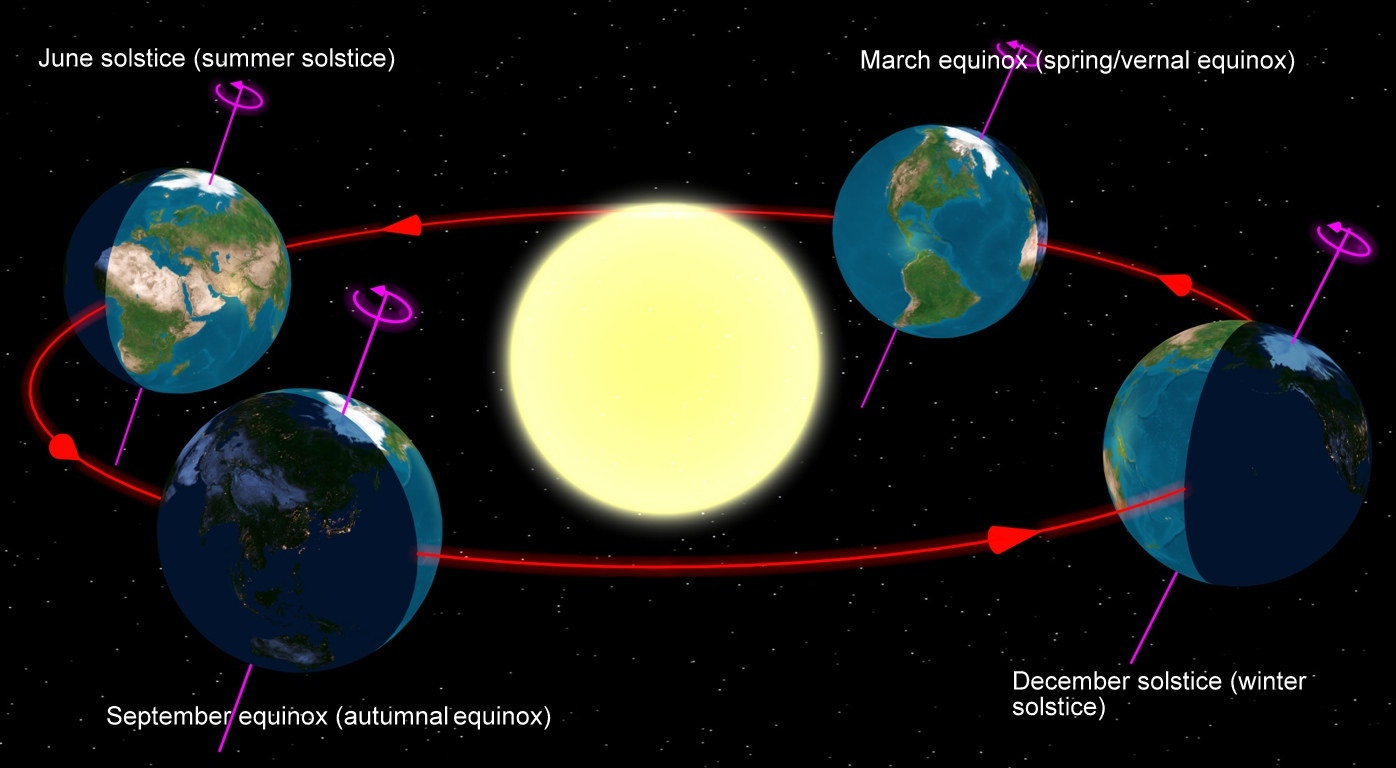
\includegraphics[width=0.6\textwidth]{solstices.jpg}

Axial tilt is why the Earth is hotter in summer. \\
It has {\color{Red}nothing} to do with the distance from the Sun!
\EC
}




\frame{\frametitle{\textbf{From last year's exam}}
\Large
What if the Earth's axial tilt were increased to $30^\circ$ from $23^\circ$?

\bigskip
\bigskip
\bigskip

\color{A}A: Syracuse would have hotter summers \\
\color{B}B: Syracuse would have colder winters \\
\color{C}C: More of Earth would be in the tropics \\
\color{D}D: More of Earth would be in the arctic \\
\color{E}E: All of the above 
}

\frame{\frametitle{\textbf{The seasons, from before}}
\BC
\Huge
Complete Lecture Tutorials pp. 93-98.

\bigskip
\bigskip
\bigskip

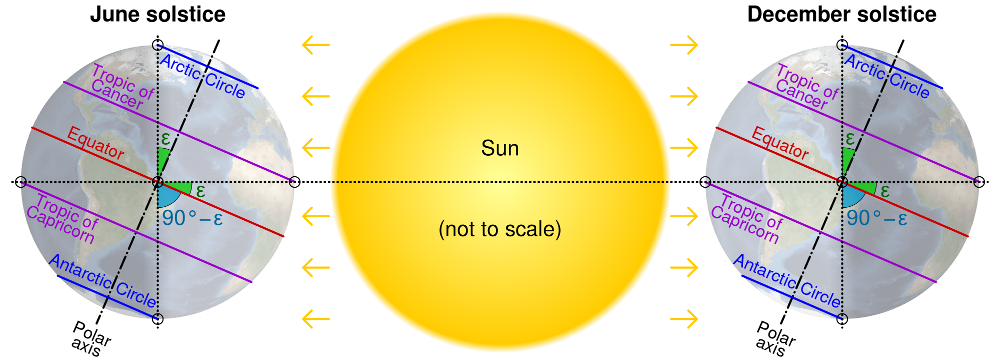
\includegraphics[width=0.8\textwidth]{circle.png}

\bigskip

\normalsize

We will talk about the Moon after this (and hear some music...)

\EC



}



\frame{

\BC
\Huge
O Fortune, like the Moon you are changeable, ever waxing and waning...

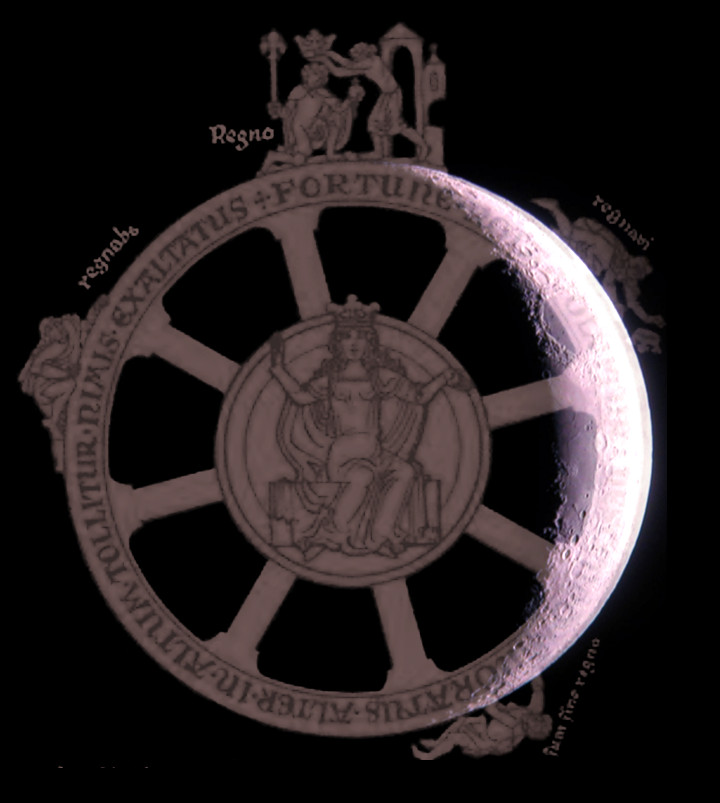
\includegraphics[width=0.4\textwidth]{Fortuna_Wheel.jpg}

O Fortuna, velut Luna, statu variabilis, semper crescis et decrescis...
\EC
}

\frame{

\begin{columns}

\column{0.5\textwidth}
O Fortune, like the Moon you are changeable, 
ever waxing and waning; hateful life 
first oppresses and then soothes
as fancy takes it; poverty and power,
it melts them like ice.

\column{0.5\textwidth}
O Fortuna, velut Luna, statu variabilis,
semper crescis aut decrescis; vita detestabilis
nunc obdurate et tunc curat 
ludo mentis aciem; egestatem, potestatem,
dissolvit ut glaciem.

\end{columns}
\pause

\bigskip
\bigskip

\begin{columns}
\column{0.5\textwidth}
Fate, monstrous and empty, you whirling wheel,
you are malevolent: wellbeing is vain 
and always fades to nothing.
Shadowed and veiled you plague me too;
now through the game I bare my back to your villainy.
\column{0.5\textwidth}
Sors immanis et inanis, rota tu volubilis,
status malus: vana salus,
semper dissolubilis.
Obumbrata et velata michi quoque niteris;
nunc per ludum dorsum nudum fero tui sceleris.
\end{columns}
\pause


\bigskip
\bigskip
\begin{columns}
\column{0.5\textwidth}
Fate is against me in health and virtue,
driven on and weighted down, always enslaved.
\column{0.5\textwidth}
Sors salutis et virtutis michi nunc contraria,
est affectus et defectus semper in angaria.
\end{columns}
\pause
\bigskip
\bigskip
\begin{columns}
\column{0.5\textwidth}
So at this hour without delay pluck the vibrating strings:
since Fate strikes down the strong,
everyone weep with me!
\column{0.5\textwidth}
Hac in hora sine mora corde pulsum tangite;
quod per sortem sternit fortem,
mecum omnes plangite!
\end{columns}
}



\frame{
\Large
From {\it Carmina Burana}, a $13^{\rm th}$-century manuscript found in an abbey south of Munich. This manuscript contained poetry written in Latin and German by
clergy in their off-duty hours, when they were decidedly not being holy!

\bigskip 

Set to music by Carl Orff (1937).

\bigskip

Other movements talk about springtime, sexuality, satire of the corrupt, drunkenness, and more sexuality;
the work both opens and closes with this movement.

}


\frame{\frametitle{\textbf{Taking stock}}
\Large
We now understand the motion of the stars, and the combined effects of the Earth's axial tilt, rotation, and orbit have on the seasons.

\bigskip
\bigskip
\bigskip

Our goal in this first segment of the course was to understand the night sky. What's left?

\BI
\item{The Moon (today)}
\item{The planets (Tuesday)}
\item{Oddities: comets, meteors, novas, eclipses... (Tuesday)}
\EI
}

\frame{\frametitle{\textbf{The phases of the Moon}}

\large

As in {\it O Fortuna}, the Moon has often been a symbol of change.

\bigskip
\bigskip
\bigskip

That change is regular, though: every 29.5 days, the pattern of phases repeats.

\bigskip
\bigskip
\bigskip

This is orderly enough that it is the basis of many calendars:

\BI
\item{Hebrew calendar}
\item{Traditional Chinese calendar}
\item{Islamic hijra calendar}
\EI

\bigskip
\bigskip
\bigskip

... but not the traditional calendars of Europe. (Why might that be?)

}

\frame{\frametitle{\textbf{The phases of the Moon}}

\large

Everything else in the sky seems to be a constant size and shape, but the Moon waxes and wanes. Why?

\pause
\bigskip
\bigskip
\bigskip

The Moon differs from the stars in that {\color{Red}it doesn't make its own light}.

\bigskip

It orbits the Earth 400,000 km (1/500 AU!) away, once every 29 days or so, orbiting counterclockwise when looking down at the North Pole.

\bigskip

What consequences does this have?

}

\frame{\frametitle{\textbf{The phases of the Moon}}

\Huge

Which is true?

\bigskip
\bigskip
\bigskip

\large

\color{A}A: The phases of the Moon happen because the Moon's motion around the Earth causes it to receive different amounts of light from the Sun, varying from completely
lit (full moon) to not lit at all (new moon) \\

\bigskip

\color{B}B: The phases of the Moon happen because half of the Moon is always lit by the Sun, but our perspective changes how much of that half we see \\

\bigskip

\color{C}C: The phases of the Moon happen because the Earth blocks part of the light from the Sun, resulting in a shadow on the Moon's face \\

\bigskip

\color{D}D: The phases of the Moon happen because the Earth moves around the Moon each day, and we see a different part of the Moon \\ 

\bigskip\pause

\color{E}E: The phases of the Moon happen because sometimes people eat the green cheese that it is made of\\
}

\frame{\frametitle{\textbf{Some new words for the moon phases...}}
\large
\BI
\item{New moon: nothing visible}
\item{Crescent: less than half visible}
\item{Half moon: half of the moon's surface is visible}
\item{Gibbous: more than half visible}
\item{Full moon: all visible}
\bigskip
\bigskip
\item{Waxing: Tomorrow the Moon will be lit more than today}
\item{Waning: Tomorrow the Moon will be lit less than today}
\EI
}

\frame{\frametitle{\textbf{How does this work?}}
\Large

\BC
\item{\color{Red} Half of the Moon is always sunlit, just like the Earth!}
\EC

\BS\BS

\BI
\item{Sometimes that half is pointed toward us: full moon!}
\item{Sometimes that half is pointed away from us: new moon!}
\EI

}

\frame{\frametitle{\textbf{How does this work?}}

\Large
\BC {\color{Red}Note that:} \EC

\BI
\large
\item Half of the Moon is always sunlit (facing toward the Sun)
\item Half of the Moon is always visible from Earth (facing toward the Earth)
\item The Moon orbits the Earth counterclockwise as seen from above the North Pole once a month
\item The Earth rotates counterclockwise as seen from the North Pole (from west to east) once a day
\EI

\BS\BS

\BC {\color{Red}To figure out the phase of the Moon:} \EC

\BI
\large
\item Draw the Earth, lunar orbit, Moon, and direction of sunlight
\item Figure out which half of the Moon is lit and label it
\item Figure out which half of the Moon we can see, and determine what it looks like
\EI

\BS\BS

\BC {\color{Red}To know when it rises and sets:} \EC
\BI
\large
\item Figure out which half of the Earth is lit and label it, to tell you night/day
\item Remember how the horizon works (I'll demonstrate)
\item This will tell you what time of day the Moon rises and sets
\EI
}

\frame{
\begin{columns}
\column{0.7\textwidth}
\BC
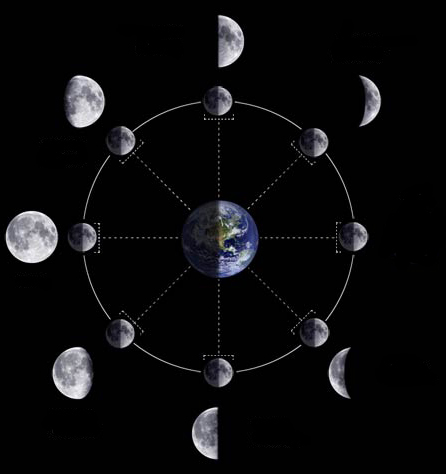
\includegraphics[width=0.95\textwidth]{phases.jpg}
\EC
\column{0.3\textwidth}
\large
You can figure all of this out by drawing pictures.

\bigskip
\bigskip
\bigskip

{\bf \color{Red}Do this} on warmup problems, tutorials, exams...

\bigskip
\bigskip
\bigskip

{\bf My desk is covered with little cartoons I drew preparing for today's class!}

\end{columns}
}

\frame{

\Huge
\BC
Complete {\it Lecture Tutorials pp. 81-84}.
\EC
}


\frame{

\Huge

When the full moon is high in the sky, it is closest to:

\bigskip
\bigskip
\bigskip

\color{A}A: 6AM \\
\color{B}B: Noon \\
\color{C}C: 6PM \\
\color{D}D: Midnight
}

\frame{

\Huge

What phase of the moon is mostly seen during the day?

\bigskip
\bigskip
\bigskip

\color{A}A: Crescent \\
\color{B}B: Full \\
\color{C}C: Half \\
\color{D}D: Gibbous
}

\frame{

\Huge \BC Complete {\it Lecture Tutorials} pp. 85-88.\EC

}

\frame{

\Huge

When the waxing half moon is just rising over the horizon, it is closest to:

\bigskip
\bigskip
\bigskip

\color{A}A: 6AM \\
\color{B}B: Noon \\
\color{C}C: 6PM \\
\color{D}D: Midnight
}

\frame{

\Huge

As seen in the Northern Hemisphere, which part of a waning crescent moon will be lit?

\bigskip
\bigskip
\bigskip

\color{A}A: The right part \\
\color{B}B: The left part \\
\color{C}C: It depends on the time of day \\

\bigskip\large
\color{white}
}


\end{document}

